\documentclass[aspectratio=169]{beamer}

% ─── Theme ────────────────────────────────────────────────────────────────────
\usetheme{Madrid}
\usecolortheme{default}
\setbeamertemplate{navigation symbols}{}
\setbeamertemplate{footline}{%
  \hfill\insertframenumber/\inserttotalframenumber\hspace*{4pt}\vspace{2pt}}

% ─── Packages ─────────────────────────────────────────────────────────────────
\usepackage{graphicx}
\usepackage{booktabs}
\usepackage{xcolor}
\usepackage{pgfplots}
\usepackage{pgfplotstable}
\usepackage{amsmath}
\usepackage{multirow}
\usepackage{array}
\usepackage{tikz}
\usepackage{hyperref}

\pgfplotsset{compat=1.18}
\usepgfplotslibrary{groupplots}
\usetikzlibrary{patterns,arrows.meta,positioning}

% ─── Colors ───────────────────────────────────────────────────────────────────
\definecolor{rdmacolor}{HTML}{E74C3C}
\definecolor{numacolor}{HTML}{2E86C1}
\definecolor{papercolor}{HTML}{27AE60}

% ─── Title ────────────────────────────────────────────────────────────────────
\title[Outback: RDMA Reproduction \& CXL Extension]{%
  Outback RDMA Key-Value Store:\\
  Reproduction, CXL Extension, and Comparative Analysis}
\author{Cheng-Shun Chuang}
\date{\today\\[4pt]
  \footnotesize\url{https://github.com/Ulrixon/outback-cxl-numa}}

\begin{document}

% ══════════════════════════════════════════════════════════════════════════════
\begin{frame}
\titlepage
\end{frame}

% ══════════════════════════════════════════════════════════════════════════════
\begin{frame}{Outline}
\tableofcontents
\end{frame}

% ══════════════════════════════════════════════════════════════════════════════
\section{Background \& Goals}
% ══════════════════════════════════════════════════════════════════════════════

\begin{frame}{What is Outback?}
\begin{columns}[T]
\column{0.50\textwidth}
\textbf{Problem:} Disaggregated memory KV stores\\
need network round-trips for every lookup.

\smallskip
\textbf{Naive:} Tree/chain indices on MN\\
$\Rightarrow$ 3--5 RDMA hops per GET

\smallskip
\textbf{Outback's insight:} Put a compact\\
\textbf{DMPH} index on every Compute Node.

\smallskip
\begin{itemize}\setlength\itemsep{2pt}
  \item CN resolves key location \textbf{locally}\\
        {\small(Othello XOR locator + per-bucket seed)}
  \item Single RPC to MN fetches value
  \item DMPH $\sim$12.5\,MB for 20M keys\\
        {\scriptsize $(2.33 + 2/\varepsilon)\!\times\!n$ bits}
\end{itemize}

\column{0.48\textwidth}
\centering
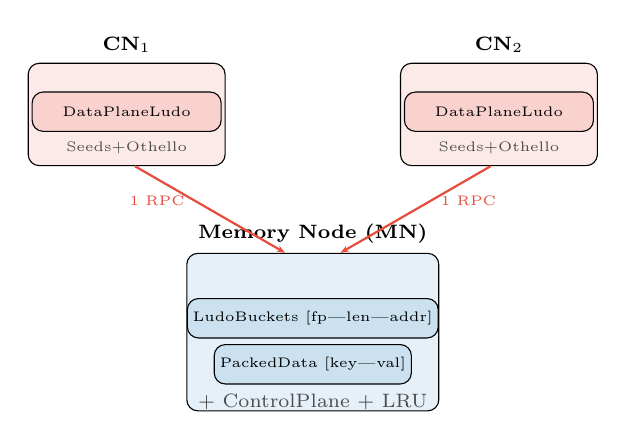
\begin{tikzpicture}[
  box/.style={draw, rounded corners, minimum width=2.4cm,
              minimum height=0.5cm, font=\scriptsize, inner sep=2pt},
  lbl/.style={font=\tiny, text=gray!60!black},
  arr/.style={-{Stealth[length=3pt]}, thick},
]
  % ── Memory Node ─────────────────
  \node[box, fill=numacolor!12, minimum height=2cm, minimum width=3.2cm,
        label={[font=\scriptsize\bfseries]above:Memory Node (MN)}] (mn) {};
  \node[box, fill=numacolor!25, font=\tiny] at ([yshift=5pt]mn.center)
        (bkt) {LudoBuckets [fp|len|addr]};
  \node[box, fill=numacolor!25, font=\tiny, below=2pt of bkt]
        (pd) {PackedData [key|val]};
  \node[lbl, below=0pt of pd] {\scriptsize + ControlPlane + LRU};

  % ── Compute Nodes ───────────────
  \node[box, fill=rdmacolor!12, minimum height=1.3cm, minimum width=2.5cm,
        above left=1.1cm and -0.5cm of mn,
        label={[font=\scriptsize\bfseries]above:CN$_1$}] (cn1) {};
  \node[box, fill=rdmacolor!25, font=\tiny] at ([yshift=1pt]cn1.center)
        (dp1) {DataPlaneLudo};
  \node[lbl, below=0pt of dp1] {Seeds+Othello};

  \node[box, fill=rdmacolor!12, minimum height=1.3cm, minimum width=2.5cm,
        above right=1.1cm and -0.5cm of mn,
        label={[font=\scriptsize\bfseries]above:CN$_2$}] (cn2) {};
  \node[box, fill=rdmacolor!25, font=\tiny] at ([yshift=1pt]cn2.center)
        (dp2) {DataPlaneLudo};
  \node[lbl, below=0pt of dp2] {Seeds+Othello};

  % ── Arrows ──────────────────────
  \draw[arr, rdmacolor] ([xshift=3pt]cn1.south) --
        node[left, font=\tiny, pos=0.4]{1 RPC} ([xshift=-10pt]mn.north);
  \draw[arr, rdmacolor] ([xshift=-3pt]cn2.south) --
        node[right, font=\tiny, pos=0.4]{1 RPC} ([xshift=10pt]mn.north);
\end{tikzpicture}
\end{columns}
\end{frame}

% ──────────────────────────────────────────────────────────────────────────────
\begin{frame}{Project Goals}
\begin{enumerate}
  \item \textbf{Reproduce} the original Outback RDMA experiments on CloudLab CX-3 nodes\\
        {\small (Xeon E5-2450, 16\,GB DDR3, MX354A CX-3 56\,Gbps FDR --- same hardware class as paper Fig.~10, 3 nodes)}
  \bigskip
  \item \textbf{Extend} Outback to a CXL-based platform by emulating CXL.mem via\\
        NUMA inter-socket shared memory on a CloudLab c6420 node\\
        {\small (2$\times$ Xeon Gold 6142, 384\,GB, UPI $\sim$100--200\,ns)}
  \bigskip
  \item \textbf{Compare} RDMA reproduction, CXL/NUMA extension, and original paper
\end{enumerate}

\vfill
\begin{block}{Why NUMA as CXL proxy?}
No dedicated CXL hardware available. Cross-socket NUMA loads/stores via UPI ($\sim$150\,ns) closely approximate CXL.mem semantics.
\end{block}
\end{frame}

% ══════════════════════════════════════════════════════════════════════════════
\section{Environment Setup}
% ══════════════════════════════════════════════════════════════════════════════

\begin{frame}{Four Platforms Compared}
\centering
\scriptsize
\begin{tabular}{@{}lcccc@{}}
\toprule
 & \textbf{Paper Fig.~9} & \textbf{Paper Fig.~10} & \textbf{RDMA Repro} & \textbf{CXL/NUMA} \\
 & \textbf{(r650)} & \textbf{(r320)} & \textbf{(r320, ours)} & \textbf{(c6420)} \\
\midrule
NIC & CX-6, 100\,Gbps & CX-3, 56\,Gbps FDR & CX-3, 56\,Gbps FDR & N/A (load/store) \\
CPU & 2$\times$Plat.~8360Y, 36C & E5-2450, 8C/16T & E5-2450, 8C/16T & 2$\times$Gold 6142, 16C \\
Memory & 256\,GB & 16\,GB & 16\,GB & 384\,GB \\
Topology & 2 shards: 1\,MN+2\,CN/shard & 1\,MN + 8\,CN & 1\,MN + 2\,CN & 1 node (NUMA) \\
MN Threads & 1/shard (Fig.~9) & 4 & 1--3 & N/A\,$^\dagger$ \\
Max CN Threads & 144/shard & 64 (8/node) & 32 (16/node) & 32 (1 socket) \\
Interconnect & 100\,Gbps IB & 56\,Gbps FDR IB & 56\,Gbps FDR IB & UPI $\sim$150\,ns \\
\bottomrule
\end{tabular}

\vspace{4pt}
\scriptsize
$^\dagger$\,CXL/NUMA has \textbf{no MN CPU}: the ``memory node'' is NUMA1 DRAM only.
CN threads (NUMA0) access it via direct \texttt{load}/\texttt{store}~--- no RPC dispatch, no MN thread.
\texttt{mem\_threads} is repurposed as \textbf{insert-lane sharding}: each value shards the
\texttt{lane\_next\_free\_index} atomic counter across $N$ lanes to reduce CAS contention on inserts.
Zero effect on reads (lookup never touches the counter); negligible on writes
because the UPI memory bus, not the counter CAS, is the actual bottleneck.

\vspace{2pt}
\small
\textbf{Our r320 $\equiv$ paper Fig.~10 hardware.} Difference: 3 nodes vs.\ 9; 1--3 MN threads vs.\ 4.\\
CXL/NUMA eliminates network entirely $\Rightarrow$ dramatically lower latency.
\end{frame}

% ══════════════════════════════════════════════════════════════════════════════
\section{CXL/NUMA Implementation}
% ══════════════════════════════════════════════════════════════════════════════

\begin{frame}{Architectural Changes: RDMA $\to$ CXL/NUMA}
\centering
\small
\begin{tabular}{@{}lll@{}}
\toprule
\textbf{Component} & \textbf{RDMA (Original)} & \textbf{CXL/NUMA (This Work)} \\
\midrule
Transport & Mellanox NIC, QPs, MRs & POSIX shm + \texttt{numa\_alloc\_onnode} \\
Execution & R2 coroutine scheduler & Direct pointer dereference \\
Concurrency & Hardware Queue Pairs & Software allocation lanes \\
Telemetry & Running-total averages & Lock-free 2D histogram \\
Lifecycle & Kernel cleans sockets & Signal handler cleanup \\
Resize & Separate branch; limited & 6-state machine, versioned epochs \\
\bottomrule
\end{tabular}

\vspace{10pt}
\begin{block}{Key insight}
Coroutine context switch ($\sim$50--100\,ns) $>$ NUMA access latency ($\sim$100--200\,ns)\\
$\Rightarrow$ Remove all coroutine logic; direct \texttt{numa\_search()} via pointer dereference
\end{block}
\end{frame}

% ══════════════════════════════════════════════════════════════════════════════
\section{Codebase Issues Discovered}
% ══════════════════════════════════════════════════════════════════════════════

\begin{frame}{Reproducibility Issues}
\begin{enumerate}
  \item \textbf{Resize on separate branch} with hard-coded 30s limits\\
        {\small Main branch runs without resizing --- different performance profile}
  \medskip
  \item \textbf{Broken zipfian for datasets} --- code accepts params but only applies to YCSB\\
        {\small Paper shows zipfian results for FB/OSM (Fig.~11c,d)}
  \medskip
  \item \textbf{Memory requirements undisclosed} --- 80M keys causes OOM during server bring-up on our 16\,GB nodes (huge-page MR + raw KV + DMPH index exhaust the huge-page pool)\\
        {\small Paper tests 80M on r650 (256\,GB)}
  \medskip
  \item \textbf{YCSB-E (range scan) unimplemented}\\
        {\small DMPH has no inherent support for ordered iteration}
  \medskip
  \item \textbf{Narrow HW compatibility} --- strict driver/kernel/NIC requirements not disclosed
  \medskip
  \item \textbf{No DMPH memory monitor} --- paper's Fig.~16 data cannot be reproduced\\
        {\small We built a custom monitor from scratch}
\end{enumerate}
\end{frame}

% ══════════════════════════════════════════════════════════════════════════════
\section{RDMA Reproduction Results}
% ══════════════════════════════════════════════════════════════════════════════

\begin{frame}{RDMA: YCSB Throughput (Paper Figs.~9--10)}
\begin{columns}[T]
% ── Left: chart ──────────────────────────────────────────────────────────────
\column{0.57\textwidth}
\centering
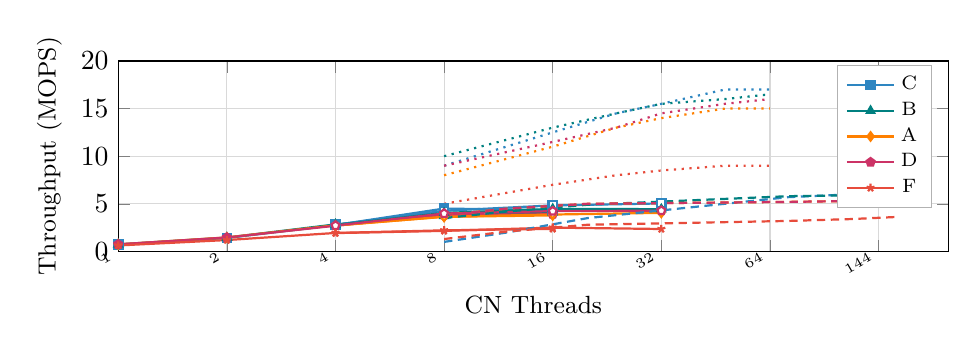
\begin{tikzpicture}
\begin{axis}[
    width=\columnwidth,
    height=4.0cm,
    ylabel={Throughput (MOPS)},
    ylabel style={font=\small},
    xlabel={CN Threads},
    xlabel style={font=\small},
    xmode=log, log basis x=2,
    xtick={1,2,4,8,16,32,64,128},
    xticklabels={1,2,4,8,16,32,64,144},
    x tick label style={rotate=30,anchor=east,font=\tiny},
    xmin=1, xmax=200,
    ymin=0, ymax=20,
    % 5-entry workload legend (style legend shown below chart)
    legend style={at={(0.98,0.98)},anchor=north east,
            font=\scriptsize,row sep=-1pt,
            fill=white,fill opacity=1,draw=black!30,text opacity=1},
    every axis plot/.append style={mark size=1.5pt, thick},
    grid=major, grid style={gray!30},
]
% Our data (1CN): filled markers, legend entries here only
\addplot[color=numacolor,mark=square*]
  coordinates {(1,0.724)(2,1.411)(4,2.770)(8,4.503)(16,4.325)};
\addlegendentry{C}
\addplot[color=teal,mark=triangle*]
  coordinates {(1,0.731)(2,1.451)(4,2.836)(8,3.722)(16,4.091)};
\addlegendentry{B}
\addplot[color=orange,mark=diamond*]
  coordinates {(1,0.740)(2,1.471)(4,2.746)(8,3.632)(16,3.783)};
\addlegendentry{A}
\addplot[color=purple!80,mark=pentagon*]
  coordinates {(1,0.744)(2,1.460)(4,2.699)(8,3.832)(16,3.900)};
\addlegendentry{D}
\addplot[color=rdmacolor,mark=star]
  coordinates {(1,0.626)(2,1.194)(4,1.939)(8,2.213)(16,2.370)};
\addlegendentry{F}
% Our data (2CN): hollow markers, same colors/shapes as 1CN
\addplot[color=numacolor,mark=square*,mark options={fill=white}]
  coordinates {(4,2.802)(8,4.269)(16,4.833)(32,5.040)};
\addplot[color=teal,mark=triangle*,mark options={fill=white}]
  coordinates {(4,2.777)(8,4.043)(16,4.461)(32,4.439)};
\addplot[color=orange,mark=diamond*,mark options={fill=white}]
  coordinates {(4,2.709)(8,3.649)(16,3.873)(32,4.049)};
\addplot[color=purple!80,mark=pentagon*,mark options={fill=white}]
  coordinates {(4,2.720)(8,3.982)(16,4.229)(32,4.281)};
\addplot[color=rdmacolor,mark=star,mark options={fill=white}]
  coordinates {(4,1.926)(8,2.157)(16,2.501)(32,2.354)};
% Paper Fig.9 (CX-6, 1MN) -- densely dashed, no legend entries
\addplot[color=numacolor,mark=none,densely dashed,thick]
  coordinates {(8,1.0)(12,2.0)(20,3.5)(72,5.7)(108,6.0)(144,6.01)};
\addplot[color=teal,mark=none,densely dashed,thick]
  coordinates {(8,3.5)(12,4.2)(20,4.9)(72,5.8)(108,5.9)(144,6.0)};
\addplot[color=orange,mark=none,densely dashed,thick]
  coordinates {(8,3.8)(12,4.5)(20,5.0)(72,5.2)(108,5.3)(144,5.5)};
\addplot[color=purple!80,mark=none,densely dashed,thick]
  coordinates {(8,3.8)(12,4.5)(20,5.0)(72,5.2)(108,5.3)(144,5.5)};
\addplot[color=rdmacolor,mark=none,densely dashed,thick]
  coordinates {(8,1.3)(12,2.1)(20,2.8)(72,3.2)(108,3.4)(144,3.62)};
% Paper Fig.10 (r320 CX-3, 4MN threads) -- dotted, no legend entries
\addplot[color=numacolor,mark=none,dotted,thick]
  coordinates {(8,9.0)(16,12.5)(24,14.5)(32,15.5)(48,17.0)(64,17.0)};
\addplot[color=teal,mark=none,dotted,thick]
  coordinates {(8,10.0)(16,13.0)(24,14.5)(32,15.5)(48,16.0)(64,16.5)};
\addplot[color=orange,mark=none,dotted,thick]
  coordinates {(8,8.0)(16,11.0)(24,13.0)(32,14.0)(48,15.0)(64,15.0)};
\addplot[color=purple!80,mark=none,dotted,thick]
  coordinates {(8,9.0)(16,11.5)(24,13.0)(32,14.5)(48,15.5)(64,16.0)};
\addplot[color=rdmacolor,mark=none,dotted,thick]
  coordinates {(8,5.0)(16,7.0)(24,8.0)(32,8.5)(48,9.0)(64,9.0)};
\end{axis}
\end{tikzpicture}

\vspace{1pt}
\begin{minipage}{\columnwidth}
\centering
{\scriptsize filled markers\,=\,ours 1\,CN (1--16\,T) \quad
 hollow markers\,=\,ours 2\,CN (4--32\,T)}\\[-1pt]
{\scriptsize dashed\,=\,Fig.~9 (6$\times$r650, CX-6, 1\,MNT/shard) \quad
 dotted\,=\,Fig.~10 (9$\times$r320, CX-3, 1\,MN+8\,CN, 4\,MNT)}
\end{minipage}

% ── Right: table + finding ────────────────────────────────────────────────────
\column{0.40\textwidth}
\centering
\scriptsize
\begin{tabular}{@{}lrrl@{}}
\toprule
\textbf{WL} & \textbf{Paper} & \textbf{Ours} & \textbf{Ratio} \\
 & \textbf{Fig.~9} & \textbf{(r320)} & \\
\midrule
C & 6.01 & 5.04 & 0.84$\times$ \\
B & 5.82 & 4.44 & 0.76$\times$ \\
A & 5.50 & 4.05 & 0.74$\times$ \\
D & 5.90 & 4.28 & 0.73$\times$ \\
F & 3.62 & 2.35 & 0.65$\times$ \\
\bottomrule
\end{tabular}

\vspace{6pt}
\begin{block}{\small Finding}
\scriptsize
65--84\% of r650 CX-6 peaks\\
despite 2$\times$ weaker NIC.\\
r320 $\equiv$ Fig.~10 hardware;\\
per-MN-thread rate consistent.
\end{block}
\end{columns}
\end{frame}

% ──────────────────────────────────────────────────────────────────────────────
\begin{frame}{RDMA: Coroutine Effect (Paper Fig.~13)}
\begin{columns}[T]
\column{0.55\textwidth}
\centering
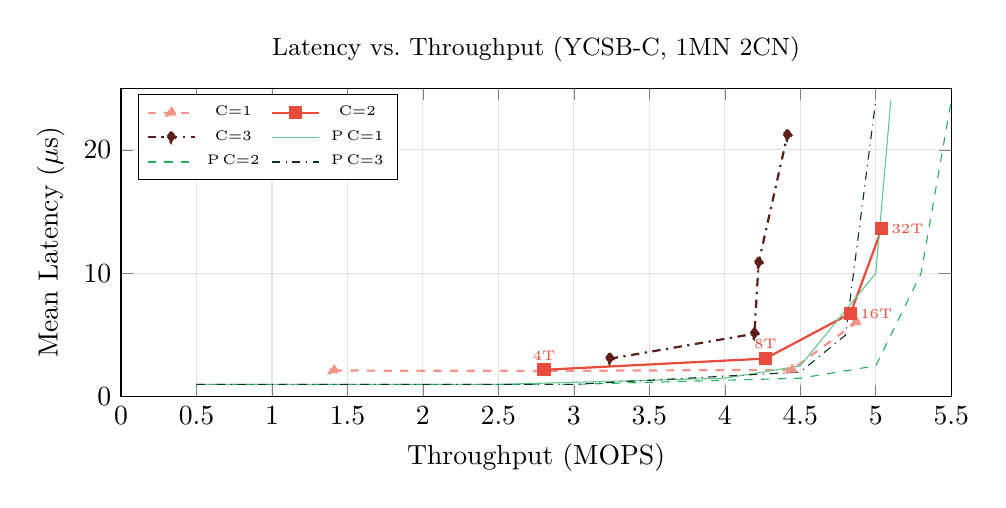
\begin{tikzpicture}
\begin{axis}[
    width=\columnwidth,
    height=5.5cm,
    xlabel={Throughput (MOPS)},
    ylabel={Mean Latency ($\mu$s)},
    xmin=0, xmax=5.5,
    ymin=0, ymax=25,
    grid=major, grid style={gray!20},
    legend style={at={(0.02,0.98)},anchor=north west,font=\tiny,
                  legend columns=2, column sep=2pt},
    every axis plot/.append style={mark size=2pt, thick},
    title style={font=\small},
    title={Latency vs.\ Throughput (YCSB-C, 1MN 2CN)}
]
% Our CX-3 data (filled markers, 1MN 2CN, 4--32 threads)
\addplot[color=rdmacolor!60,mark=triangle*,dashed]
  coordinates {(1.409,2.12)(2.808,2.09)(4.443,2.18)(4.870,6.01)};
\addplot[color=rdmacolor,mark=square*]
  coordinates {(2.802,2.18)(4.269,3.09)(4.833,6.75)(5.040,13.63)};
\addplot[color=rdmacolor!40!black,mark=diamond*,dashdotted]
  coordinates {(3.238,3.08)(4.196,5.10)(4.224,10.85)(4.414,21.18)};
% Paper Fig.~13a (CX-6, MT=1, digitized) -- thin green overlay
\addplot[color=papercolor!70,mark=none,thin]
  coordinates {(0.5,1.0)(2.5,1.0)(4.0,1.5)(4.5,2.5)(5.0,10)(5.1,24)};
\addplot[color=papercolor,mark=none,thin,dashed]
  coordinates {(0.5,1.0)(3.0,1.0)(4.5,1.5)(5.0,2.5)(5.3,10)(5.5,24)};
\addplot[color=papercolor!30!black,mark=none,thin,dashdotted]
  coordinates {(0.5,1.0)(3.0,1.0)(4.5,2.0)(4.8,5.0)(5.0,24)};
\legend{C=1, C=2, C=3, P\,C=1, P\,C=2, P\,C=3}
% Thread-count labels on C=2 curve
\node[font=\tiny,anchor=south,rdmacolor] at (axis cs:2.802,2.18) {4T};
\node[font=\tiny,anchor=south,rdmacolor] at (axis cs:4.269,3.09) {8T};
\node[font=\tiny,anchor=west,rdmacolor]  at (axis cs:4.833,6.75) {16T};
\node[font=\tiny,anchor=west,rdmacolor]  at (axis cs:5.040,13.63) {32T};
\end{axis}
\end{tikzpicture}

\column{0.42\textwidth}
\begin{itemize}
  \item \textbf{``Hockey stick'':} flat latency\\
        until saturation, then explodes
  \bigskip
  \item Paper (thin green) baseline\\
        $\sim$1\,$\mu$s vs.\ ours $\sim$2\,$\mu$s\\
        (CX-6 vs.\ CX-3 NIC)
  \bigskip
  \item Our C=2 peaks at 5.04\,MOPS;\\
        paper $\sim$5.5\,MOPS
  \bigskip
  \item C=3 peaks lower (4.41\,MOPS):\\
        excess queue depth on\\
        saturated MN degrades tput
  \bigskip
  \item Both platforms: same shape
\end{itemize}
\end{columns}
\end{frame}

% ══════════════════════════════════════════════════════════════════════════════
\section{CXL/NUMA Results}
% ══════════════════════════════════════════════════════════════════════════════

\begin{frame}{CXL/NUMA: All YCSB Workloads}
\centering
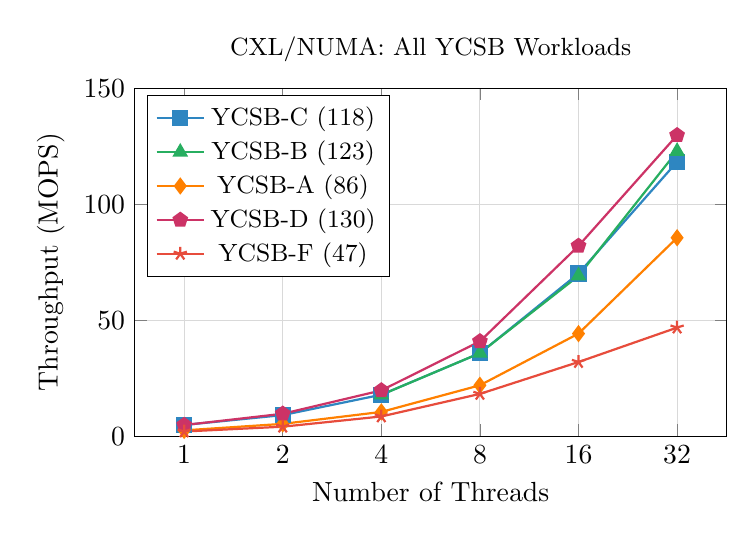
\begin{tikzpicture}
\begin{axis}[
    width=0.75\textwidth,
    height=6cm,
    ylabel={Throughput (MOPS)},
    xlabel={Number of Threads},
    xmode=log, log basis x=2,
    xtick={1,2,4,8,16,32},
    xticklabels={1,2,4,8,16,32},
    ymin=0, ymax=150,
    legend style={at={(0.02,0.98)},anchor=north west,font=\small},
    every axis plot/.append style={mark size=2.5pt, thick},
    grid=major, grid style={gray!30},
    title style={font=\small},
    title={CXL/NUMA: All YCSB Workloads}
]
\addplot[color=numacolor,mark=square*]
  coordinates {(1,4.794)(2,9.056)(4,17.833)(8,35.737)(16,70.091)(32,118.270)};
\addplot[color=papercolor,mark=triangle*]
  coordinates {(4,17.775)(8,35.772)(16,69.087)(32,122.821)};
\addplot[color=orange,mark=diamond*]
  coordinates {(1,2.470)(2,5.269)(4,10.422)(8,21.909)(16,44.183)(32,85.514)};
\addplot[color=purple!80,mark=pentagon*]
  coordinates {(1,4.764)(2,9.628)(4,19.691)(8,40.854)(16,82.002)(32,129.707)};
\addplot[color=rdmacolor,mark=star]
  coordinates {(1,1.970)(2,4.051)(4,8.460)(8,18.189)(16,31.935)(32,46.775)};
\legend{YCSB-C (118), YCSB-B (123), YCSB-A (86), YCSB-D (130), YCSB-F (47)}
\end{axis}
\end{tikzpicture}

\vspace{4pt}
Read-dominated (C, B, D) scale past 100\,MOPS. Write-heavy YCSB-F plateaus at 47\,MOPS.
\end{frame}

% ══════════════════════════════════════════════════════════════════════════════
\section{Three-Way Comparison}
% ══════════════════════════════════════════════════════════════════════════════

\begin{frame}{Three-Way: YCSB-C Throughput Scaling}
\centering
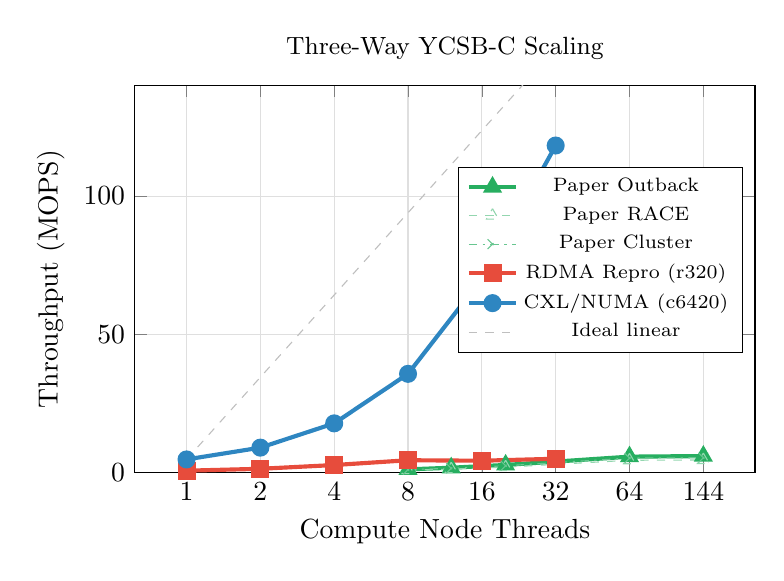
\begin{tikzpicture}
\begin{axis}[
    width=0.78\textwidth,
    height=6.5cm,
    ylabel={Throughput (MOPS)},
    xlabel={Compute Node Threads},
    xmode=log, log basis x=2,
    xtick={1,2,4,8,16,32,64,128},
    xticklabels={1,2,4,8,16,32,64,144},
    ymin=0, ymax=140,
    legend style={at={(0.98,0.55)},anchor=east,font=\scriptsize},
    every axis plot/.append style={mark size=2.5pt, thick},
    grid=major, grid style={gray!25},
    title style={font=\small},
    title={Three-Way YCSB-C Scaling}
]
\addplot[color=papercolor,mark=triangle*,line width=1.5pt]
  coordinates {(8,1.2)(12,1.8)(20,2.8)(64,5.8)(128,6.01)};
\addplot[color=papercolor!50,mark=triangle,dashed,thin]
  coordinates {(8,0.9)(12,1.3)(20,2.0)(64,4.5)(128,4.59)};
\addplot[color=papercolor!70,mark=x,dashdotted,thin]
  coordinates {(8,1.1)(12,1.6)(20,2.5)(64,5.3)(128,5.41)};
\addplot[color=rdmacolor,mark=square*,line width=1.5pt]
  coordinates {(1,0.724)(2,1.411)(4,2.770)(8,4.503)(16,4.325)(32,5.040)};
\addplot[color=numacolor,mark=*,line width=1.5pt]
  coordinates {(1,4.794)(2,9.056)(4,17.833)(8,35.737)(16,70.091)(32,118.270)};
\addplot[color=gray!50,dashed,no marks,thin]
  coordinates {(1,4.794)(32,153.408)};
\legend{Paper Outback, Paper RACE, Paper Cluster, RDMA Repro (r320), CXL/NUMA (c6420), Ideal linear}
\end{axis}
\end{tikzpicture}

Paper Outback, RACE, Cluster all plateau at 4.5--6\,MOPS (MN CPU bound). CXL/NUMA scales linearly.
\end{frame}

% ──────────────────────────────────────────────────────────────────────────────
\begin{frame}{Three-Way: Peak Throughput (All YCSB)}
\centering
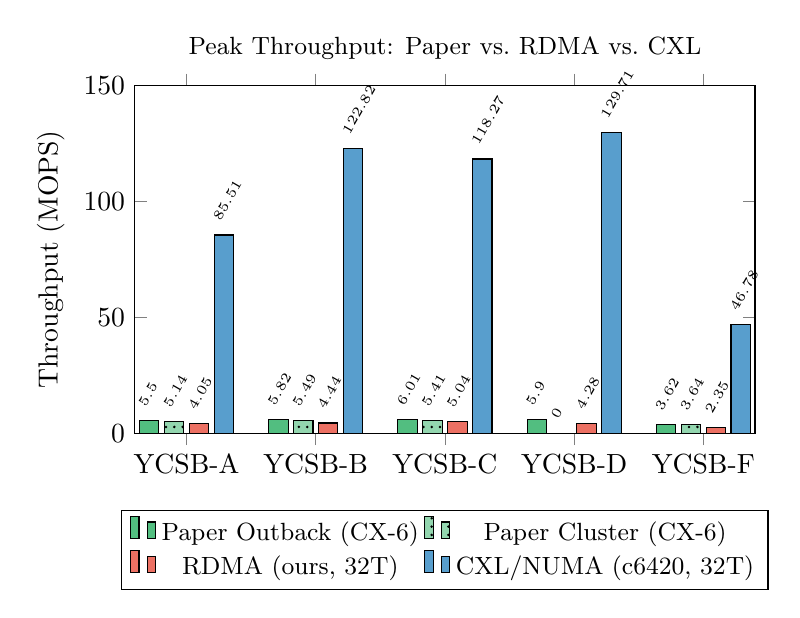
\begin{tikzpicture}
\begin{axis}[
    ybar,
    width=0.78\textwidth,
    height=6cm,
    ylabel={Throughput (MOPS)},
    symbolic x coords={YCSB-A,YCSB-B,YCSB-C,YCSB-D,YCSB-F},
    xtick=data,
    ymin=0, ymax=150,
    bar width=7pt,
    legend style={at={(0.5,-0.22)},anchor=north,legend columns=2,font=\small},
    nodes near coords,
    nodes near coords style={font=\tiny,rotate=60,anchor=south west},
    title style={font=\small},
    title={Peak Throughput: Paper vs.\ RDMA vs.\ CXL}
]
\addplot[fill=papercolor!80] coordinates {
  (YCSB-A,5.50)(YCSB-B,5.82)(YCSB-C,6.01)(YCSB-D,5.90)(YCSB-F,3.62)
};
\addplot[fill=papercolor!50,postaction={pattern=dots}] coordinates {
  (YCSB-A,5.14)(YCSB-B,5.49)(YCSB-C,5.41)(YCSB-D,0)(YCSB-F,3.64)
};
\addplot[fill=rdmacolor!80] coordinates {
  (YCSB-A,4.05)(YCSB-B,4.44)(YCSB-C,5.04)(YCSB-D,4.28)(YCSB-F,2.35)
};
\addplot[fill=numacolor!80] coordinates {
  (YCSB-A,85.51)(YCSB-B,122.82)(YCSB-C,118.27)(YCSB-D,129.71)(YCSB-F,46.78)
};
\legend{Paper Outback (CX-6), Paper Cluster (CX-6), RDMA (ours{,} 32T), CXL/NUMA (c6420{,} 32T)}
\end{axis}
\end{tikzpicture}

CXL/NUMA achieves \textbf{15--22$\times$} the paper's peak with 4.5$\times$ fewer threads.
\end{frame}

% ──────────────────────────────────────────────────────────────────────────────
\begin{frame}{Three-Way: Latency vs.\ Throughput}
\centering
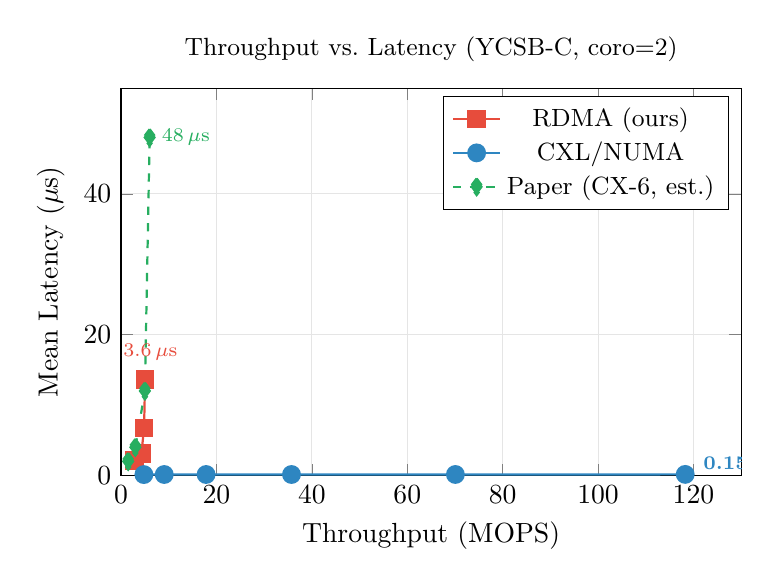
\begin{tikzpicture}
\begin{axis}[
    width=0.78\textwidth,
    height=6.5cm,
    xlabel={Throughput (MOPS)},
    ylabel={Mean Latency ($\mu$s)},
    xmin=0, xmax=130,
    ymin=0, ymax=55,
    grid=major, grid style={gray!20},
    title style={font=\small},
    title={Throughput vs.\ Latency (YCSB-C, coro=2)},
    legend style={at={(0.98,0.98)},anchor=north east,font=\small},
    mark size=3pt,
]
\addplot[color=rdmacolor,mark=square*,thick] coordinates {
  (2.802,2.18)(4.269,3.09)(4.833,6.75)(5.040,13.63)
};
\addlegendentry{RDMA (ours)}
\addplot[color=numacolor,mark=*,thick] coordinates {
  (4.794,0.126)(9.056,0.135)(17.833,0.137)(35.737,0.139)(70.091,0.141)(118.270,0.153)
};
\addlegendentry{CXL/NUMA}
\addplot[color=papercolor,mark=diamond*,thick,dashed] coordinates {
  (1.5,2.0)(3.0,4.0)(5.0,12.0)(6.0,48.0)
};
\addlegendentry{Paper (CX-6, est.)}

\node[font=\scriptsize,anchor=west,numacolor] at (axis cs:120,1.5) {\textbf{0.15\,$\mu$s}};
\node[font=\scriptsize,anchor=south,rdmacolor] at (axis cs:5.0,15) {13.6\,$\mu$s};
\node[font=\scriptsize,anchor=west,papercolor] at (axis cs:6.5,48) {48\,$\mu$s};
\end{axis}
\end{tikzpicture}

CXL: \textbf{both} higher throughput and lower latency. No throughput--latency trade-off.
\end{frame}

% ──────────────────────────────────────────────────────────────────────────────
\begin{frame}{Three-Way: MN Thread Scalability (Paper Fig.~12)}
\begin{columns}[T]
\column{0.55\textwidth}
\centering
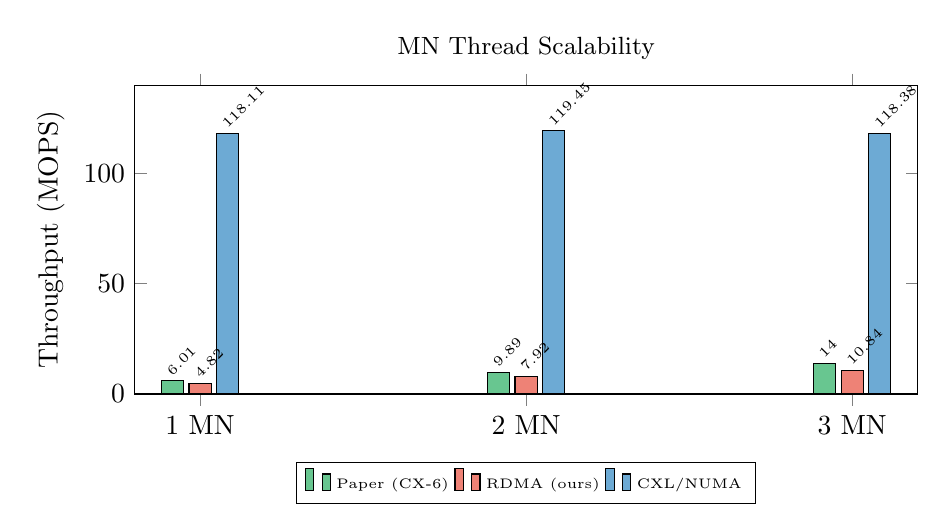
\begin{tikzpicture}
\begin{axis}[
    ybar,
    width=0.95\columnwidth,
    height=5.5cm,
    ylabel={Throughput (MOPS)},
    symbolic x coords={{1 MN},{2 MN},{3 MN}},
    xtick=data,
    ymin=0, ymax=140,
    bar width=8pt,
    legend style={at={(0.5,-0.22)},anchor=north,legend columns=3,font=\tiny},
    nodes near coords,
    nodes near coords style={font=\tiny,rotate=45,anchor=south west,inner sep=1pt},
    title style={font=\small},
    title={MN Thread Scalability}
]
\addplot[fill=papercolor!70] coordinates {
  ({1 MN},6.01)({2 MN},9.89)({3 MN},14.0)
};
\addplot[fill=rdmacolor!70] coordinates {
  ({1 MN},4.82)({2 MN},7.92)({3 MN},10.84)
};
\addplot[fill=numacolor!70] coordinates {
  ({1 MN},118.11)({2 MN},119.45)({3 MN},118.38)
};
\legend{Paper (CX-6), RDMA (ours), CXL/NUMA}
\end{axis}
\end{tikzpicture}

\column{0.42\textwidth}
\begin{itemize}
  \item Paper \& RDMA: throughput\\
        scales $\sim$linearly with MN threads
  \bigskip
  \item CXL/NUMA: \textbf{flat} at 118\,MOPS\\
        regardless of MN threads
  \bigskip
  \item Root cause: RDMA requires\\
        MN CPU for RPC dispatch
  \bigskip
  \item CXL: no server-side CPU\\
        involved $\Rightarrow$ no MN bottleneck
\end{itemize}
\end{columns}
\end{frame}

% ──────────────────────────────────────────────────────────────────────────────
\begin{frame}{CXL/NUMA: Coroutines Are Irrelevant}
\begin{columns}[T]
\column{0.52\textwidth}
\centering
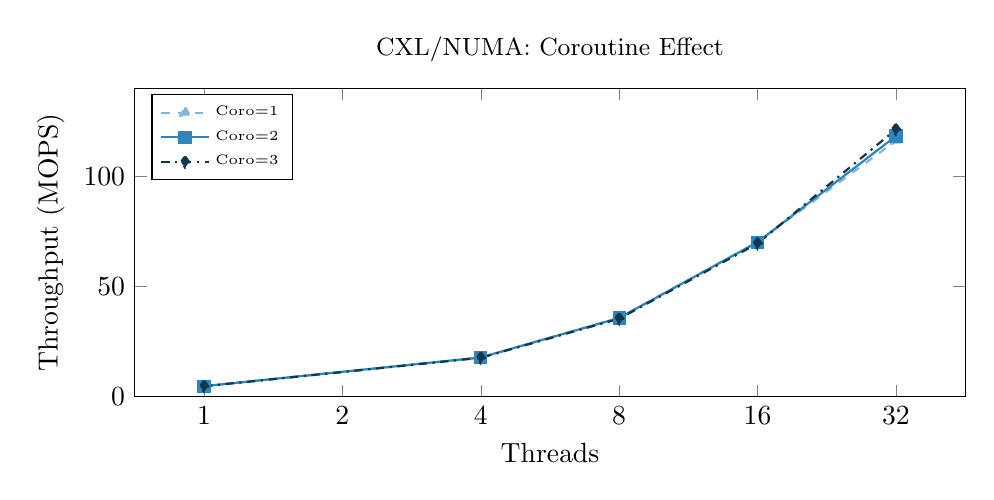
\begin{tikzpicture}
\begin{axis}[
    width=\columnwidth,
    height=5.5cm,
    ylabel={Throughput (MOPS)},
    xlabel={Threads},
    xmode=log, log basis x=2,
    xtick={1,2,4,8,16,32},
    xticklabels={1,2,4,8,16,32},
    ymin=0, ymax=140,
    legend style={at={(0.02,0.98)},anchor=north west,font=\tiny},
    every axis plot/.append style={mark size=2pt, thick},
    title style={font=\small},
    title={CXL/NUMA: Coroutine Effect}
]
\addplot[color=numacolor!60,mark=triangle*,dashed]
  coordinates {(1,4.776)(4,17.734)(8,35.827)(16,70.214)(32,116.106)};
\addplot[color=numacolor,mark=square*]
  coordinates {(1,4.794)(4,17.833)(8,35.737)(16,70.091)(32,118.270)};
\addplot[color=numacolor!40!black,mark=diamond*,dashdotted]
  coordinates {(1,4.743)(4,17.675)(8,35.399)(16,69.548)(32,121.286)};
\legend{Coro=1, Coro=2, Coro=3}
\end{axis}
\end{tikzpicture}

\column{0.45\textwidth}
\begin{itemize}
  \item All three curves \textbf{overlap perfectly}
  \bigskip
  \item Latency: 0.13--0.15\,$\mu$s\\
        regardless of coro count
  \bigskip
  \item NUMA latency ($\sim$150\,ns): coroutine\\
        switch ($\sim$50--100\,ns) not amortized
  \bigskip
  \item $\Rightarrow$ No latency to hide\\
        $\Rightarrow$ Coroutines are pure overhead
  \bigskip
  \item \textbf{Contrast:} RDMA needs coro=2\\
        for 2$\times$ throughput gain
\end{itemize}
\end{columns}
\end{frame}

% ──────────────────────────────────────────────────────────────────────────────
\begin{frame}{Resize Behavior: RDMA \& CXL/NUMA}
\begin{columns}[T]
\column{0.50\textwidth}
\centering
{\small\textbf{RDMA (CX-3, 20M keys, YCSB-D)}}\\[2pt]
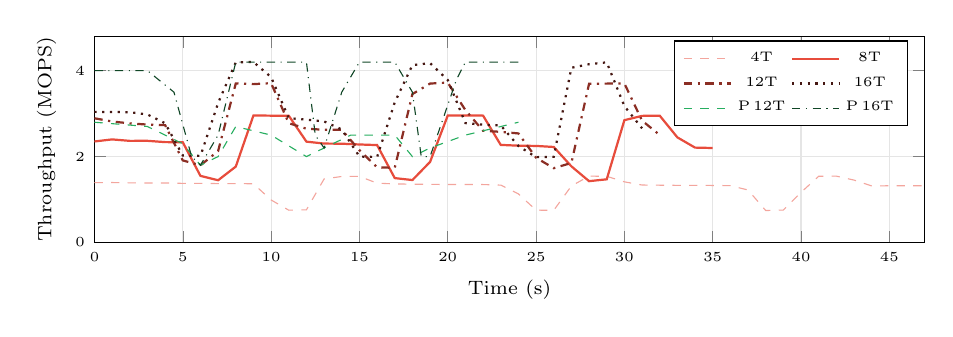
\begin{tikzpicture}
\begin{axis}[
    width=\columnwidth,
    height=4.2cm,
    ylabel={Throughput (MOPS)},
    xlabel={Time (s)},
    ymin=0, ymax=4.8,
    xmin=0, xmax=47,
    grid=major, grid style={gray!20},
    legend style={at={(0.98,0.98)},anchor=north east,font=\tiny,legend columns=2},
    tick label style={font=\tiny},
    ylabel style={font=\scriptsize},
    xlabel style={font=\scriptsize},
]
\addplot[color=rdmacolor!50,mark=none,dashed] coordinates {
  (0,1.394)(1,1.396)(2,1.389)(3,1.384)(4,1.386)(5,1.377)
  (6,1.378)(7,1.371)(8,1.372)(9,1.367)(10,0.990)(11,0.752)
  (12,0.761)(13,1.480)(14,1.537)(15,1.540)(16,1.381)(17,1.364)
  (18,1.358)(19,1.353)(20,1.350)(21,1.351)(22,1.349)(23,1.336)
  (24,1.131)(25,0.753)(26,0.749)(27,1.316)(28,1.545)(29,1.541)
  (30,1.412)(31,1.338)(32,1.334)(33,1.331)(34,1.330)(35,1.328)
  (36,1.324)(37,1.222)(38,0.744)(39,0.755)(40,1.167)(41,1.542)
  (42,1.545)(43,1.453)(44,1.316)(45,1.321)(46,1.320)(47,1.321)
};
\addlegendentry{4T}
\addplot[color=rdmacolor,mark=none,thick] coordinates {
  (0,2.352)(1,2.400)(2,2.366)(3,2.367)(4,2.337)(5,2.333)
  (6,1.551)(7,1.449)(8,1.767)(9,2.957)(10,2.953)(11,2.952)
  (12,2.348)(13,2.303)(14,2.300)(15,2.282)(16,2.268)
  (17,1.499)(18,1.454)(19,1.877)(20,2.955)(21,2.959)(22,2.954)
  (23,2.272)(24,2.254)(25,2.248)(26,2.224)
  (27,1.773)(28,1.428)(29,1.471)(30,2.848)(31,2.948)(32,2.953)
  (33,2.447)(34,2.209)(35,2.200)
};
\addlegendentry{8T}
\addplot[color=rdmacolor!60!black,mark=none,thick,dashdotted] coordinates {
  (0,2.892)(1,2.817)(2,2.773)(3,2.745)(4,2.732)
  (5,1.911)(6,1.796)(7,2.129)(8,3.702)(9,3.687)(10,3.710)
  (11,2.778)(12,2.649)(13,2.624)(14,2.622)
  (15,2.149)(16,1.751)(17,1.738)(18,3.456)(19,3.700)(20,3.723)
  (21,3.082)(22,2.601)(23,2.576)(24,2.539)
  (25,1.974)(26,1.730)(27,1.852)(28,3.694)(29,3.699)(30,3.703)
  (31,2.836)(32,2.503)
};
\addlegendentry{12T}
\addplot[color=rdmacolor!30!black,mark=none,thick,dotted] coordinates {
  (0,3.041)(1,3.037)(2,3.034)(3,2.980)
  (4,2.776)(5,2.025)(6,2.016)(7,3.249)(8,4.193)(9,4.202)
  (10,3.850)(11,2.895)(12,2.860)(13,2.818)
  (14,2.632)(15,2.001)(16,1.990)(17,3.263)(18,4.130)(19,4.175)
  (20,3.783)(21,2.780)(22,2.742)(23,2.727)
  (24,2.247)(25,1.987)(26,1.994)(27,4.068)(28,4.151)(29,4.194)
  (30,3.176)(31,2.658)
};
\addlegendentry{16T}
\addplot[color=papercolor,mark=none,thin,dashed] coordinates {
  (0,2.8)(3,2.7)(5,2.3)(6,1.8)(7,2.0)(8,2.7)(10,2.5)
  (12,2.0)(13,2.2)(14.5,2.5)(17,2.5)
  (18,2.0)(19,2.2)(21,2.5)(24,2.8)};
\addlegendentry{P\,12T}
\addplot[color=papercolor!40!black,mark=none,thin,dashdotted] coordinates {
  (0,4.0)(3,4.0)(4.5,3.5)(5.5,2.0)(6,1.8)(7,2.5)(8,4.2)(12,4.2)
  (12.5,2.5)(13,2.2)(14,3.5)(15,4.2)(17,4.2)
  (18,3.5)(18.5,2.0)(19,2.0)(20.5,3.8)(21,4.2)(24,4.2)};
\addlegendentry{P\,16T}
\end{axis}
\end{tikzpicture}
{\tiny Erratic post-resize spikes $\pm$38\% vs.\ paper's smooth $\sim$52\% dip}

\column{0.50\textwidth}
\centering
{\small\textbf{CXL/NUMA (c6420, 20M keys, YCSB-D)}}\\[2pt]
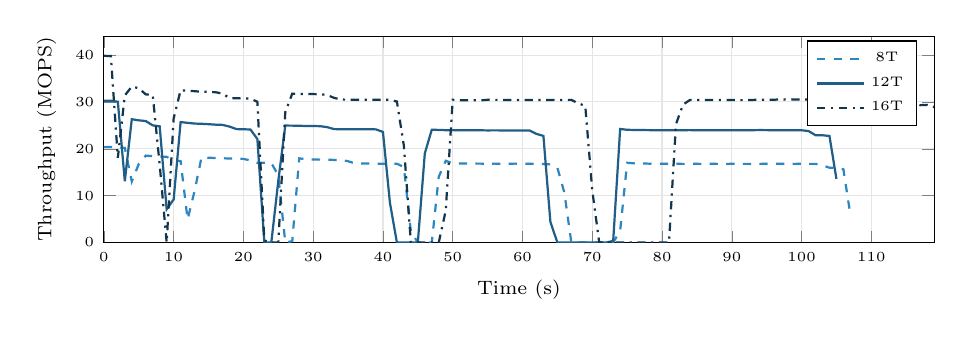
\begin{tikzpicture}
\begin{axis}[
    width=\columnwidth,
    height=4.2cm,
    ylabel={Throughput (MOPS)},
    xlabel={Time (s)},
    ymin=0, ymax=44,
    xmin=0, xmax=119,
    grid=major, grid style={gray!20},
    legend style={at={(0.98,0.98)},anchor=north east,font=\tiny},
    tick label style={font=\tiny},
    ylabel style={font=\scriptsize},
    xlabel style={font=\scriptsize},
]
\addplot[color=numacolor,mark=none,thick,dashed] coordinates {
  (0,20.35)(1,20.39)(2,20.27)(3,20.19)(4,13.02)(5,16.74)
  (6,18.54)(7,18.42)(8,18.35)(9,18.28)(10,17.55)(11,17.36)
  (12,4.92)(13,10.99)(14,18.21)(15,18.09)(16,18.03)(17,17.97)
  (18,17.93)(19,17.88)(20,17.84)(21,17.51)(22,17.02)(23,17.01)
  (24,16.98)(25,14.31)(26,0)(27,0.28)(28,17.95)(29,17.78)
  (30,17.72)(31,17.68)(32,17.68)(33,17.62)(34,17.59)(35,17.35)
  (36,16.86)(37,16.85)(38,16.84)(39,16.82)(40,16.81)(41,16.80)
  (42,16.81)(43,16.11)(44,2.38)(45,0)(46,0)(47,0)
  (48,14.03)(49,17.43)(50,16.90)(51,16.88)(52,16.86)(53,16.84)
  (54,16.83)(55,16.81)(56,16.83)(57,16.81)(58,16.82)(59,16.83)
  (60,16.79)(61,16.80)(62,16.79)(63,16.77)(64,16.66)(65,15.98)
  (66,10.66)(67,0)(68,0)(69,0)(70,0)(71,0)
  (72,0)(73,0)(74,2.46)(75,17.01)(76,16.89)(77,16.87)
  (78,16.83)(79,16.81)(80,16.82)(81,16.79)(82,16.79)(83,16.78)
  (84,16.79)(85,16.79)(86,16.76)(87,16.79)(88,16.78)(89,16.77)
  (90,16.79)(91,16.77)(92,16.78)(93,16.77)(94,16.78)(95,16.79)
  (96,16.79)(97,16.81)(98,16.79)(99,16.78)(100,16.79)(101,16.78)
  (102,16.78)(103,16.47)(104,15.96)(105,15.99)(106,15.62)(107,5.89)
};
\addlegendentry{8T}
\addplot[color=numacolor!70!black,mark=none,thick] coordinates {
  (0,30.23)(1,30.25)(2,30.04)(3,13.08)(4,26.31)(5,26.07)
  (6,25.92)(7,25.00)(8,24.79)(9,7.10)(10,9.18)(11,25.71)
  (12,25.53)(13,25.38)(14,25.33)(15,25.25)(16,25.15)(17,25.10)
  (18,24.74)(19,24.20)(20,24.16)(21,24.12)(22,22.09)(23,0)
  (24,0)(25,13.14)(26,24.95)(27,24.94)(28,24.91)(29,24.86)
  (30,24.86)(31,24.82)(32,24.62)(33,24.20)(34,24.17)(35,24.19)
  (36,24.15)(37,24.18)(38,24.18)(39,24.14)(40,23.59)(41,8.49)
  (42,0)(43,0)(44,0)(45,0)(46,19.01)(47,24.08)
  (48,24.02)(49,23.97)(50,23.98)(51,23.95)(52,23.94)(53,23.95)
  (54,23.94)(55,23.92)(56,23.93)(57,23.92)(58,23.91)(59,23.90)
  (60,23.90)(61,23.92)(62,23.18)(63,22.75)(64,4.41)(65,0)
  (66,0)(67,0)(68,0)(69,0)(70,0)(71,0)
  (72,0)(73,0.33)(74,24.23)(75,24.05)(76,24.02)(77,24.00)
  (78,23.98)(79,23.96)(80,23.94)(81,23.97)(82,23.95)(83,23.97)
  (84,23.98)(85,23.95)(86,23.96)(87,23.96)(88,23.95)(89,23.96)
  (90,23.94)(91,23.97)(92,23.97)(93,23.97)(94,23.99)(95,23.98)
  (96,23.96)(97,23.97)(98,23.97)(99,23.95)(100,23.95)(101,23.78)
  (102,22.90)(103,22.88)(104,22.74)(105,13.57)
};
\addlegendentry{12T}
\addplot[color=numacolor!40!black,mark=none,thick,dashdotted] coordinates {
  (0,39.84)(1,39.79)(2,18.07)(3,31.38)(4,33.28)(5,32.92)
  (6,31.61)(7,31.47)(8,16.58)(9,0)(10,26.47)(11,32.50)
  (12,32.38)(13,32.29)(14,32.17)(15,32.14)(16,32.07)(17,31.79)
  (18,30.82)(19,30.79)(20,30.73)(21,30.70)(22,30.03)(23,0.42)
  (24,0)(25,0)(26,27.82)(27,31.77)(28,31.70)(29,31.70)
  (30,31.67)(31,31.64)(32,31.49)(33,30.86)(34,30.51)(35,30.47)
  (36,30.44)(37,30.47)(38,30.43)(39,30.47)(40,30.48)(41,30.43)
  (42,30.09)(43,20.64)(44,0)(45,0)(46,0)(47,0)
  (48,0)(49,6.82)(50,30.46)(51,30.36)(52,30.34)(53,30.34)
  (54,30.34)(55,30.45)(56,30.44)(57,30.43)(58,30.41)(59,30.42)
  (60,30.42)(61,30.42)(62,30.41)(63,30.39)(64,30.42)(65,30.40)
  (66,30.42)(67,30.44)(68,29.69)(69,29.15)(70,11.15)(71,0)
  (72,0)(73,0)(74,0)(75,0)(76,0)(77,0)
  (78,0)(79,0)(80,0)(81,0)(82,25.24)(83,29.40)
  (84,30.42)(85,30.40)(86,30.43)(87,30.42)(88,30.41)(89,30.42)
  (90,30.41)(91,30.38)(92,30.39)(93,30.43)(94,30.47)(95,30.45)
  (96,30.46)(97,30.55)(98,30.49)(99,30.52)(100,30.52)(101,30.49)
  (102,30.50)(103,30.50)(104,30.49)(105,30.49)(106,30.48)(107,30.48)
  (108,30.48)(109,30.51)(110,30.50)(111,30.48)(112,30.56)(113,30.61)
  (114,30.57)(115,30.65)(116,29.89)(117,29.31)(118,29.35)(119,28.92)
};
\addlegendentry{16T}
\end{axis}
\end{tikzpicture}
{\tiny $\sim$95\% stall for 1--12\,s; 16T stall $\sim$12\,s at high table occupancy}
\end{columns}
\end{frame}

% ──────────────────────────────────────────────────────────────────────────────
\begin{frame}{Memory Usage: Paper vs.\ Reality --- LF\,=\,0.80, 0.85, 0.90 \& 0.95}
\begin{columns}[T]
\column{0.50\textwidth}
\centering
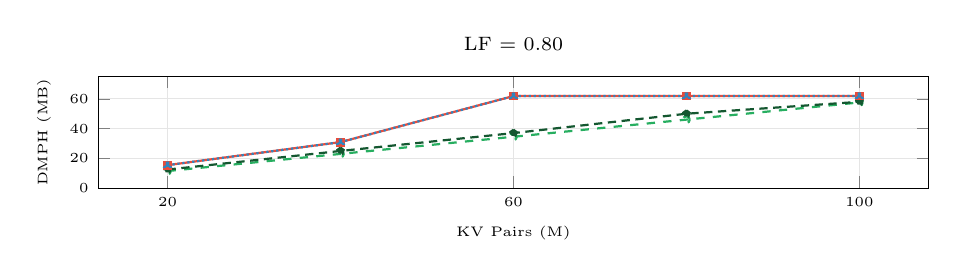
\begin{tikzpicture}
\begin{axis}[
    width=\columnwidth, height=3.0cm,
    xlabel={KV Pairs (M)}, xlabel style={font=\tiny},
    ylabel={DMPH (MB)}, ylabel style={font=\tiny},
    xtick={20,60,100}, ymin=0, ymax=75,
    grid=major, grid style={gray!20},
    tick label style={font=\tiny},
    every axis plot/.append style={thick},
    title style={font=\scriptsize}, title={LF = 0.80}
]
\addplot[color=papercolor,dashed,mark=o,mark size=1.2pt]
  coordinates {(20,11.52)(40,23.03)(60,34.55)(80,46.06)(100,57.58)};
\addplot[color=papercolor!50!black,densely dashed,mark=pentagon*,mark size=1.2pt]
  coordinates {(20,12.5)(40,25)(60,37)(80,50)(100,58)};
\addplot[color=rdmacolor,mark=square*,mark size=1.2pt]
  coordinates {(20,15.48)(40,30.95)(60,61.88)(80,61.88)(100,61.88)};
\addplot[color=numacolor,mark=triangle*,mark size=1.2pt,densely dotted]
  coordinates {(20,15.47)(40,30.93)(60,61.87)(80,61.87)(100,61.87)};
\end{axis}
\end{tikzpicture}

\vspace{4pt}
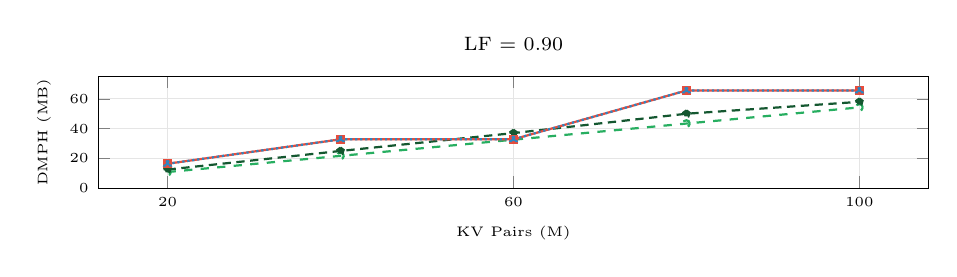
\begin{tikzpicture}
\begin{axis}[
    width=\columnwidth, height=3.0cm,
    xlabel={KV Pairs (M)}, xlabel style={font=\tiny},
    ylabel={DMPH (MB)}, ylabel style={font=\tiny},
    xtick={20,60,100}, ymin=0, ymax=75,
    grid=major, grid style={gray!20},
    tick label style={font=\tiny},
    every axis plot/.append style={thick},
    title style={font=\scriptsize}, title={LF = 0.90}
]
\addplot[color=papercolor,dashed,mark=o,mark size=1.2pt]
  coordinates {(20,10.85)(40,21.71)(60,32.56)(80,43.41)(100,54.27)};
\addplot[color=papercolor!50!black,densely dashed,mark=pentagon*,mark size=1.2pt]
  coordinates {(20,12.5)(40,25)(60,37)(80,50)(100,58)};
\addplot[color=rdmacolor,mark=square*,mark size=1.2pt]
  coordinates {(20,16.42)(40,32.82)(60,32.82)(80,65.62)(100,65.62)};
\addplot[color=numacolor,mark=triangle*,mark size=1.2pt,densely dotted]
  coordinates {(20,16.40)(40,32.80)(60,32.80)(80,65.60)(100,65.60)};
\end{axis}
\end{tikzpicture}

\column{0.50\textwidth}
\centering
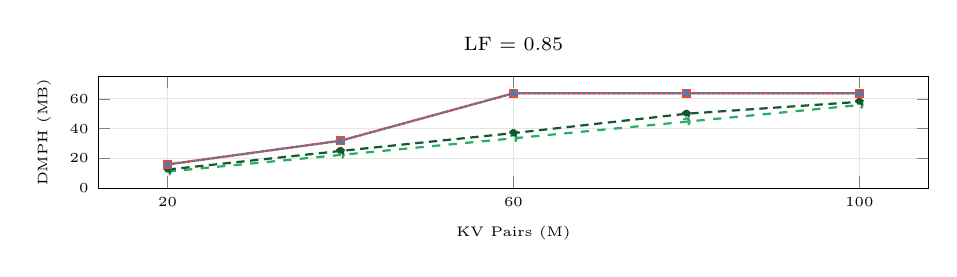
\begin{tikzpicture}
\begin{axis}[
    width=\columnwidth, height=3.0cm,
    xlabel={KV Pairs (M)}, xlabel style={font=\tiny},
    ylabel={DMPH (MB)}, ylabel style={font=\tiny},
    xtick={20,60,100}, ymin=0, ymax=75,
    grid=major, grid style={gray!20},
    tick label style={font=\tiny},
    every axis plot/.append style={thick},
    title style={font=\scriptsize}, title={LF = 0.85}
]
\addplot[color=papercolor,dashed,mark=o,mark size=1.2pt]
  coordinates {(20,11.17)(40,22.33)(60,33.50)(80,44.66)(100,55.83)};
\addplot[color=papercolor!50!black,densely dashed,mark=pentagon*,mark size=1.2pt]
  coordinates {(20,12.5)(40,25)(60,37)(80,50)(100,58)};
\addplot[color=rdmacolor,mark=square*,mark size=1.2pt]
  coordinates {(20,15.95)(40,31.88)(60,63.75)(80,63.75)(100,63.75)};
\addplot[color=numacolor,mark=triangle*,mark size=1.2pt,densely dotted]
  coordinates {(20,15.93)(40,31.87)(60,63.73)(80,63.73)(100,63.73)};
\end{axis}
\end{tikzpicture}

\vspace{4pt}
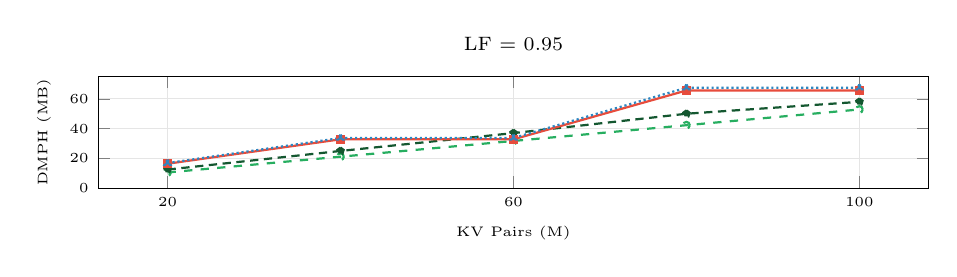
\begin{tikzpicture}
\begin{axis}[
    width=\columnwidth, height=3.0cm,
    xlabel={KV Pairs (M)}, xlabel style={font=\tiny},
    ylabel={DMPH (MB)}, ylabel style={font=\tiny},
    xtick={20,60,100}, ymin=0, ymax=75,
    grid=major, grid style={gray!20},
    tick label style={font=\tiny},
    every axis plot/.append style={thick},
    title style={font=\scriptsize}, title={LF = 0.95}
]
\addplot[color=papercolor,dashed,mark=o,mark size=1.2pt]
  coordinates {(20,10.57)(40,21.15)(60,31.72)(80,42.30)(100,52.87)};
\addplot[color=papercolor!50!black,densely dashed,mark=pentagon*,mark size=1.2pt]
  coordinates {(20,12.5)(40,25)(60,37)(80,50)(100,58)};
\addplot[color=rdmacolor,mark=square*,mark size=1.2pt]
  coordinates {(20,16.42)(40,32.82)(60,32.82)(80,65.62)(100,65.62)};
\addplot[color=numacolor,mark=triangle*,mark size=1.2pt,densely dotted]
  coordinates {(20,16.87)(40,33.73)(60,33.73)(80,67.47)(100,67.47)};
\end{axis}
\end{tikzpicture}
\end{columns}

\vspace{2pt}
\centering\scriptsize
\textcolor{papercolor}{--- Formula} \quad \textcolor{papercolor!50!black}{--$\bullet$ Fig.16} \quad \textcolor{rdmacolor}{$\blacksquare$ RDMA} \quad \textcolor{numacolor}{$\blacktriangle$ CXL} \hfill
Power-of-2 allocation $\Rightarrow$ step-wise jumps; LF$\leq$0.85: 60M jump $\sim$\textbf{72\% over} paper
\end{frame}

% ══════════════════════════════════════════════════════════════════════════════
\section{Key Findings Summary}
% ══════════════════════════════════════════════════════════════════════════════

\begin{frame}{Reproduction vs.\ Paper: Discrepancy Summary}
\centering
\small
\begin{tabular}{@{}p{3cm}p{3cm}p{5.5cm}@{}}
\toprule
\textbf{Paper Claim} & \textbf{Published} & \textbf{Our Finding} \\
\midrule
5.03$\times$ over RACE & CX-3, YCSB-C & Consistent per-MN-thread rate \\
6.01\,MOPS peak & CX-6, 144T & 5.04 on CX-3 (0.84$\times$); CXL: 118 \\
Linear scaling & To 144T & Saturates at $\sim$5\,MOPS (MN bound) \\
Smooth resize & $\sim$52\% drop & 45\% RDMA / 95\% CXL (brief stall) \\
12.5\,MB/20M keys & Fig.~16 & 16.87\,MB; process RSS: 915.8\,MB \\
Write performance & Competitive & YCSB-F degrades at 32T \\
Code completeness & Implied & Separate resize branch; broken zipfian; no YCSB-E \\
\bottomrule
\end{tabular}
\end{frame}

% ══════════════════════════════════════════════════════════════════════════════
\section{Discussion \& Conclusion}
% ══════════════════════════════════════════════════════════════════════════════

\begin{frame}{CXL Advantages \& Limitations}
\begin{columns}[T]
\column{0.48\textwidth}
\textcolor{numacolor}{\textbf{Advantages}}
\begin{enumerate}
  \item \textbf{Latency:} 0.14\,$\mu$s vs.\ 3\,$\mu$s\\
        (15--20$\times$ improvement)
  \medskip
  \item \textbf{Scalability:} linear with threads\\
        (no shared NIC bottleneck)
  \medskip
  \item \textbf{Simplicity:} no coroutines,\\
        no QP management, no MRs\\
        ($\sim$60\% less code complexity)
  \medskip
  \item \textbf{Memory efficiency:}\\
        no RDMA buffer registration
\end{enumerate}

\column{0.48\textwidth}
\textcolor{rdmacolor}{\textbf{Limitations}}
\begin{enumerate}
  \item \textbf{Single-machine scope}\\
        (needs CXL~3.0 for multi-node)
  \medskip
  \item \textbf{Write contention:}\\
        cache-line bouncing without\\
        HW QP offloading
  \medskip
  \item \textbf{Resize stalls:}\\
        atomic remap blocks all clients
  \medskip
  \item \textbf{Cleanup required:}\\
        signal handlers for /dev/shm
\end{enumerate}
\end{columns}
\end{frame}

% ──────────────────────────────────────────────────────────────────────────────
\begin{frame}{Conclusion}
\begin{block}{Reproduction}
RDMA reproduction on r320 (same hardware class as paper Fig.~10) \textbf{confirms} per-MN-thread throughput trends but reveals:\\
undisclosed memory overhead, write degradation, codebase incompleteness.
\end{block}

\begin{block}{CXL Extension}
CXL/NUMA port achieves \textbf{118\,MOPS} (23$\times$ RDMA) with \textbf{0.14\,$\mu$s} latency (21$\times$ lower).\\
Near-linear scaling with no NIC bottleneck demonstrates CXL is a fundamentally\\
superior transport for DMPH-indexed KV stores.
\end{block}

\begin{block}{Next Steps}
\begin{itemize}\setlength{\itemsep}{0pt}
  \item Validate on real CXL hardware (Samsung CXL memory expander)
  \item Explore multi-node CXL pooling (CXL~3.0)
  \item Reproduce paper's baselines (RACE, MICA) for direct ratio verification
  \item Write-heavy optimizations (software write-combining for YCSB-F)
\end{itemize}
\end{block}
\end{frame}

% ══════════════════════════════════════════════════════════════════════════════
\begin{frame}{}
\centering
\vfill
{\Huge\textbf{Thank You}}\\[12pt]
{\Large Questions?}
\vfill
\end{frame}

% ══════════════════════════════════════════════════════════════════════════════
\appendix
\begin{frame}{Appendix}
\centering
{\Large Backup Slides}
\end{frame}

% ──────────────────────────────────────────────────────────────────────────────
\begin{frame}{Resize State Machine}
\centering
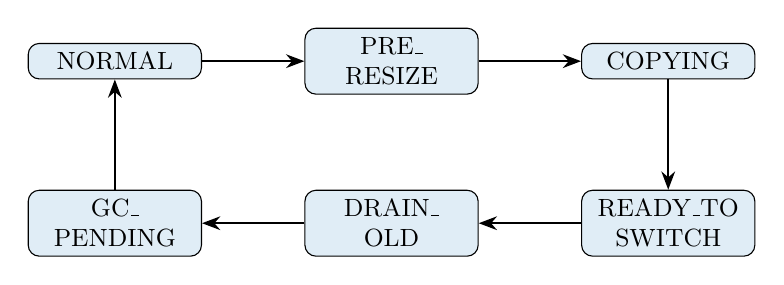
\begin{tikzpicture}[
  state/.style={draw, rounded corners, fill=numacolor!15, minimum width=2.2cm, font=\small, align=center},
  arr/.style={-{Stealth}, thick},
  node distance=1.4cm and 1.3cm
]
  \node[state] (n) {NORMAL};
  \node[state, right=of n] (pr) {PRE\_\\RESIZE};
  \node[state, right=of pr] (cp) {COPYING};
  \node[state, below=of cp] (rs) {READY\_TO\\SWITCH};
  \node[state, left=of rs] (dr) {DRAIN\_\\OLD};
  \node[state, left=of dr] (gc) {GC\_\\PENDING};

  \draw[arr] (n) -- (pr);
  \draw[arr] (pr) -- (cp);
  \draw[arr] (cp) -- (rs);
  \draw[arr] (rs) -- (dr);
  \draw[arr] (dr) -- (gc);
  \draw[arr] (gc) -- (n);
\end{tikzpicture}

\vspace{8pt}
\begin{itemize}
  \item Each epoch creates a new versioned shared-memory region
  \item Clients detect changes via generation counter, transparently remap
  \item Mutations deferred during COPYING/DRAIN, replayed after switch
\end{itemize}
\end{frame}

% ──────────────────────────────────────────────────────────────────────────────
\begin{frame}{DMPH Lookup: How One-Hop Works}
\centering
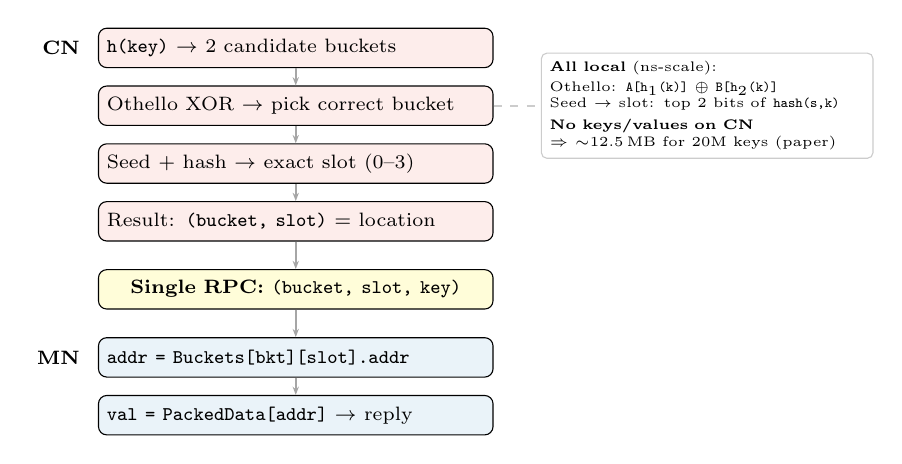
\begin{tikzpicture}[
  stepbox/.style={draw, rounded corners=3pt, minimum height=0.5cm,
               font=\scriptsize, inner sep=3pt, text width=4.8cm, align=left},
  lbl/.style={font=\scriptsize\bfseries, anchor=east},
  arr/.style={-{Stealth[length=3pt]}, thick, gray!70},
  node distance=0.22cm,
]
  % CN steps
  \node[stepbox, fill=rdmacolor!10] (s1)
        {\texttt{h(key)} $\to$ 2 candidate buckets};
  \node[lbl, left=3pt of s1] {CN};
  \node[stepbox, fill=rdmacolor!10, below=of s1] (s2)
        {Othello XOR $\to$ pick correct bucket};
  \node[stepbox, fill=rdmacolor!10, below=of s2] (s3)
        {Seed + hash $\to$ exact slot (0--3)};
  \node[stepbox, fill=rdmacolor!10, below=of s3] (s4)
        {Result: \texttt{(bucket, slot)} = location};

  % Network
  \node[stepbox, fill=yellow!15, below=0.35cm of s4, text width=4.8cm, align=center] (net)
        {\textbf{Single RPC:} \texttt{(bucket, slot, key)}};

  % MN steps
  \node[stepbox, fill=numacolor!10, below=0.35cm of net] (m1)
        {\texttt{addr = Buckets[bkt][slot].addr}};
  \node[lbl, left=3pt of m1] {MN};
  \node[stepbox, fill=numacolor!10, below=of m1] (m2)
        {\texttt{val = PackedData[addr]} $\to$ reply};

  % Arrows
  \foreach \a/\b in {s1/s2, s2/s3, s3/s4, s4/net, net/m1, m1/m2}
    \draw[arr] (\a) -- (\b);

  % Annotation
  \node[right=0.6cm of s2, font=\tiny, text width=4cm, align=left,
        fill=white, draw=gray!40, rounded corners=2pt, inner sep=3pt] (ann)
    {\textbf{All local} (ns-scale):\\[1pt]
     Othello: \texttt{A[h$_1$(k)] $\oplus$ B[h$_2$(k)]}\\
     Seed $\to$ slot: top 2 bits of \texttt{hash(s,k)}\\[2pt]
     \textbf{No keys/values on CN}\\
     $\Rightarrow$ $\sim$12.5\,MB for 20M keys (paper)};
  \draw[gray!40, thick, dashed] (s2.east) -- (ann.west);

\end{tikzpicture}

\vspace{4pt}
\small
\textbf{vs.\ baselines:} RACE needs 2--3 hops (hash chain); tree indices need $O(\log n)$ traversals
\end{frame}

\end{document}
